\documentclass{article}
\usepackage[T1]{fontenc}
\usepackage[utf8]{inputenc}
\usepackage{lmodern}
\usepackage{textgreek}
\usepackage{amsmath}
\usepackage{mathtools}
\usepackage{graphicx}
\usepackage{spconf}

\usepackage{tabularx}
\usepackage{blindtext}
\usepackage{hyperref}
\usepackage{pgfgantt}
\usepackage{colortbl}
\usepackage{pdfpages}
\usepackage{setspace}
\usepackage{booktabs}

\setcounter{tocdepth}{3}

\title{Applied machine learning system ELEC0134 20/21 report}
\name{SN: 17139494}
\address{}

\begin{document}
\maketitle

\begin{abstract}
\iffalse
This section provides a brief overview of the methodology/results
presented in the report.
\fi
This report describes methodology of solving four tasks using machine learning. The aim is to find optimal method that is computationally efficient and has reasonable accuracy. First two tasks are based on celebrity face image dataset and is requires classifying gender and smile. Both tasks use Haar Cascade Classifier and Dlib face detection to locate faces in image. It was chosen to use CNN for first task, which has achieved 92\% accuracy on test dataset. Second task was implemented by extracting facial landmarks and trained on SVM achieving 88.8\% accuracy on test data.  Third and fourth tasks are based on cartoon face images and requires to classify one of five face shapes and eye colours. Third task had almost no preprocessing and downscaled grey images were directly fed to SVM algorithm achieving 99.96\% accuracy. Fourth task required custom method to discard images faces with completely obscuring glasses. This discarded about 18.6\% of images, which were further classified using Random Forest Classifier achieving 99.361\% accuracy on test dataset. \footnote{The code is provided in\\ \href{https://github.com/zceemja/AMLS_ASSIGNMENT_20-21}{github.com/zceemja/AMLS\_ASSIGNMENT\_20-21}}
\end{abstract}

\section{Introduction}
\label{sec:intro}
\iffalse
This section introduces the problem, a brief bird’s-eye view
of the methodologies you adopted and the organization of this
report.
\fi
In the past ten years machine learning has increasingly dominated more and more sectors to solve and optimise problems previously thought would be too complex to tackle. It has achieved this by training a generic algorithm on data extracted for the read world which results in accurately predicting output from never before seen data. This enables to solve complex problems much easier, reducing development time and/or reduce needed computing power to solve problem, as suppose to hand-crafting algorithm manually that reliably work for every edge case scenario. One of the examples is complex physics simulations that can trained with neural network can accurately predict particle movements with 2 to 5 orders of magnitude computation time reduction enabling real-time applications \cite{Zsolnai13fc,physics}. This shift from manual writing code and applying machine learning to a problem is also referred as software 2.0 \cite{software2}. 

In this report four problems will be solved using two similar datasets — images of celebrity and cartoon faces. Each task will tackle different classification problem:
\\\\
\begin{description}
	\item[Task A1:] Classify binary gender with celebrity faces;
	\item[Task A2:] Classify if person is smiling with celebrity faces;
	\item[Task B1:] Classify one of five different cartoon face shapes;
	\item[Task B2:] Classify one of five different cartoon character eye colour.
\end{description}
Problems defined in task will be attempted to solved using machine learning techniques. Aim is to select most optimal model in terms of computation speed, training time and prediction accuracy. For this reason a model with lower accuracy, as long as accuracy is still reasonable; would be preferred over a model that is substantially longer to compute prediction or train the model itself.

Report is further section in reviewing existing know methods and potential approaches in \autoref{sec:lite}, model descriptions used to solve each problem in \autoref{sec:models}, implemententation methods and code in \autoref{sec:impl}, results of the best models and accuracy of previously not-seen data in \autoref{sec:results} and summary \& future improvements in \autoref{sec:conc}.   
\section{Literature Survey}
\label{sec:lite}
\iffalse
This section should focus on an overview of potential ap-
proaches to solve the tasks. You can introduce some classical
and state-of-the-art machine learning algorithms.

09148181 - Gender classifier using CNN
08298719 - Gender classifier based on GoogLeNet
05170659 - Gneder classifier with SVM and landmarks, multiregion. 
06391660 - Gender classifier with Haar Cascade, it looks for moustache, beard, and general classifier.
07554002 - Gender classifier from 3D faces and random forest.
04959635 - Gender classifier using RFV, nonlinear SVM, pretty good paper

08578838 - Smile generator using landmarks.
08349659 - Improvements of smile detection with adaboost. Can use smile to estimate gender.
00670950 - importance of in eye and mouth movements to classify smiles.
08620951 - Gender classifier with CNN, performance varies with illumination, poses, occlusion, rotation
08398872 - Gender detection with CNN and running on RPI
\fi
A number of methods for gender classification from facial images have been published throughout years, newer papers suggesting novel configurations to improve upon accuracy and performance. 

Article \cite{4959635} introduces Rectangle Feature Vector (RFV) learned by AdaBoost with combination of nonlinear Support Vector Machine (SVM) for gender identification. This paper introduces quite novel method with relatively good results and small dataset of 1,759 images. Training methods seem to be quite difficult to implement in python due to need of writing a lot of custom code, however data preprocessing is explained quite well. It aligns and crops mouth centred images, and normalises to size of $24 \times 24$, further performing histogram equalization. 

Article \cite{5170659} divides face into multiple region and show that upper face region  is the most important to identify gender, however they propose a method to use a number of regions (not all face) approach trained with SVM to improve accuracy. This approach could be implemented in task A1 to improve accuracy.

Similarly, article \cite{6391660} extracts facial features from images using Haar Cascade Classifiers and uses a number of tricks to improve processing time such as first detecting moustache or beard to identify male gender with lower complexity SVM model, and further use more complex general gender classifier. Furthermore, it extracts parts face regions and uses Weber features images to increase SVM model accuracy 

Article \cite{9148181} uses Convolutional Neural Network to solve gender classification problem. It compares various networks such as VGG16, Inception V3 and ResNet50 showing that highest accuracy was achieved with VGG16 network that is the smallest out of three of them with 16M tunable parameters. 

Article \cite{8398872} also tackles gender classification problem using CNN, and they describe custom network implementation with tensorflow in python. This model is efficient enough to working on lower power Raspberry Pi 3 model B+. CNN used in task A1 is highly inspired by this paper.

Article \cite{8620951} uses CNN and some other preprocessing methods such as facial landmark extraction to rotate image making eyes align horizontally. Also it crops various patches of the same face to increase dataset and make network more robust to occlusion.

A number of articles \cite{8578838,670950} explore facial expressions of smiles and show that other facial parts than mouth such as eyes and cheeks are also important to determinate if person is smiling. 

Article \cite{8349659} explores two other papers using Eigen face and Fisher face methods for smile detection. It uses AdaBoost to achieve better performance of these two novel methods. It is a useful article to that compares two smile detection methods that could be used in task A2, and how they can be further improved. 

Article \cite{7789587} uses general-to-specific fine-tuning scheme and strategies that exploit inherit correlation in data to detect both gender and smile. It also uses a number of preprocessing methods such as face alignment, and uses VGG-Faces CNN model.

\section{Description Of Models}
\label{sec:models}
\iffalse
In this section, you should briefly describe the model you are
using for each task, along with the rationale. You may opt to
use a single learning algorithm to solve the problem or multi-
ple ones, but bear in mind there are page limitations and that
you should explain your rationale behind your choices. That
is, the algorithmic description must detail your reasons for
selecting a particular model.
You can clarify them with flow charts, figures or equa-
tions.
\fi


\subsection{Task A1: Gender classification}

To implement gender classification CNN was used. In literature review there are a number of papers that use both CNN and SVM to solve this problem, however the trade-off with SVM is that it requires more preprocessing and more implementation to achieve high accuracy whereas CNN is easier to implement, achieves better accuracy and task has sufficiently large dataset to be trained on. 

Structure of implemented CNN is described in \autoref{tab:a1_cnn}.
\begin{figure}[htb]
	\centering
	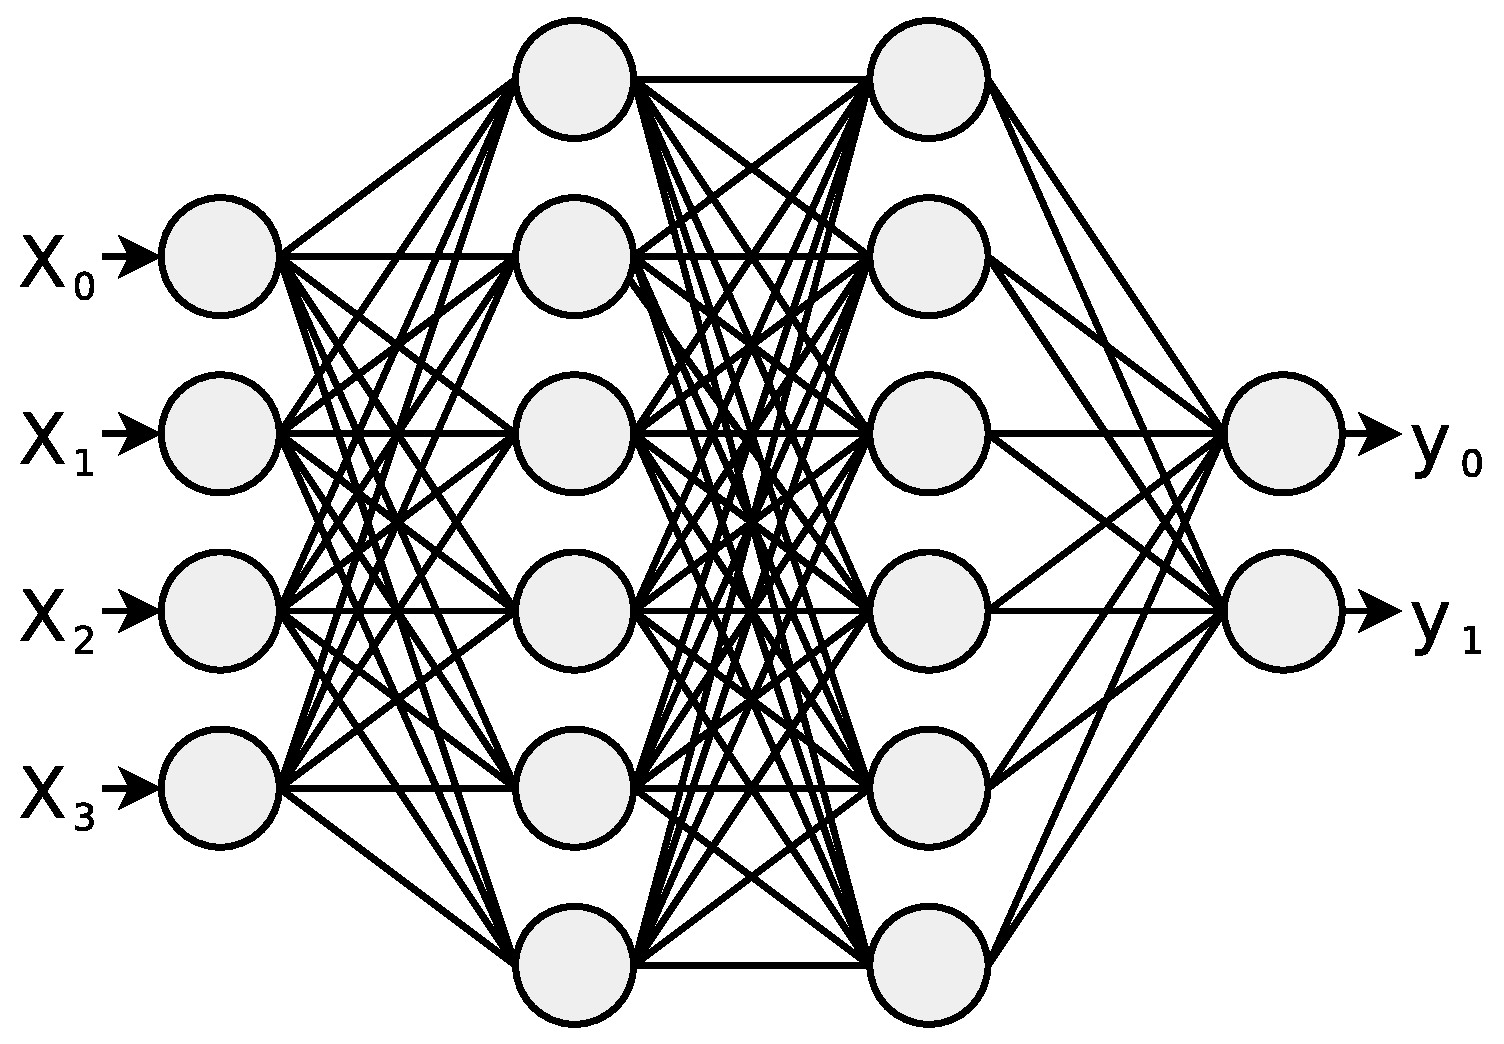
\includegraphics[width=0.5\linewidth]{graphics/NN.eps}
	\caption{A generic structure of Artifical Nerual Network.}
	\label{fig:general_nn}	
\end{figure}
\autoref{fig:general_nn} shows a structure of neural network. It has layers seen as columns of neurons shown as circles. In this case it has input of four tensors and output of two. Each neuron is connected to each neural of the next layer using a synapse that contains weigh. All neurons perform operation shown in \autoref{eq:nn}.
\begin{equation}\label{eq:nn}
	y_{j,k} = f\left( \sum_{i=0} x_{i,k-1} W_{i,k} + B_{j,k} \right)
\end{equation}
Where $y_{j,k}$ is output of neuron, $f()$ is activation function, $B_{j,k}$ is neuron bias value, $x_{i,k-1}$ are outputs from previous layer neurons and $W_{i,k}$ synapse weight. In this task ReLU activation is used which has formula of $f(x) = \max(0, x)$ and last layer has Softmax activation which has formula in \autoref{eq:softmax}.
\begin{equation}\label{eq:softmax}
	f(\pmb{x})_i = \frac{e^{x_i}}{\sum_{j=1}^{K}e^{x_j}}
\end{equation}

In addition, first two layers of implemented CNN uses convolutional layer that makes input image abstracted to some feature map.
Pooling layers combines small clusters of size $2 \times 2$ and selects the highest value out of local cluster.
Flatten layer converts 2-dimensional data structure to a 1D vector.
Dropout layer randomly dropout with probability of 0.2 during training stage. This reduces model overfitting. 

\subsection{Task A2: Smile classification}
\label{sub:svm}
A number of models for each task are tested with specific hyper-parameters. Implementation of finding model and hyper-parameters are described in \autoref{sub:hypertune}. Task A2 selected SVM with Radial Basis Function (RBF) kernel because though testing it provided the highest accuracy. SVM is supervised machine learning models that maps training data to points in some space in such way to maximise the gap between different data classes. When new data is tested, it is also mapped to points in the same space and category is selected depending on which side of the gap point is. Kernel defines how these points are placed by mapping them to some higher dimensional space. Two additional hyper-parameters are used — gamma which defines how far the influence of single training point reaches. Other parameter C trade off classification accuracy and simplicity of decision function. 

A CNN model could be also applied to face images this task however SVM was selected due to very simple model with only 136 vector inputs with acceptable accuracy.
\subsection{Task B1: Face shape classification}
As with task A2, a number of models with different hyper-parameters were tested as described in \autoref{sub:hypertune}. Most of the models showed very high accuracy only applying histogram equalization and downscaling on images. 

Highest accuracy provided SVM model with polynomial kernel. This kernel is fairly simple with polynomial definition shown in \autoref{eq:poly}.
\begin{equation}\label{eq:poly}
	K(\pmb{x},\pmb{y}) = (\pmb{x}^\top\pmb{y}+c)^d
\end{equation}
$x$ and $y$ are points in space, d is degree of polynomial, and c is another hyper-parameter.
No other methods have been explored because of already high model accuracy. 

\subsection{Task B2: Eye colour classification}
As described before, best model was selected using implementation in \autoref{sub:hypertune}. 
Random Forest was used as it produced the best accuracy. Unlike SVM, random forest constructs decision trees that contain a number of functions that decide on class. Number of trees in forest is set as a hyper-parameter. Each tree outputs decision on a single class and forest picks the class that most trees have selected. Random Forest Classifier was used instead of other Decision Tree Classifiers because of it suffer less from overfitting.

The accuracy of this model is very high and complexity is optimal therefore no further models has been explored. 

\section{Implementation}
\label{sec:impl}
\iffalse
This section must provide the detailed implementation of your
models. In particular, you must provide the name and use of
external libraries, explain hyper-parameter selection, training
pipeline (if any) and key modules/classes/functions/algorithms.
You also must provide a detailed description of the dataset
(content, size, format, etc.), any data pre-processing that was
applied and how you separate your dataset into training, vali-
dation and test sets.
The execution of your models also should be reported
here. In particular, this section should include a thorough dis-
cussion on the training convergence and stopping criterion (it
is recommended that learning curves graphs be used to this
effect).
\fi

\subsection{Parent Model Class}
\label{sub:parent_class}
Each task is constructed to be a class that is initialised in \textit{main.py}. \texttt{tune\_model, train, test, cleanup} methods are executed from \textit{main.py} too. Each model class has a common parent class located in \textit{Common/common.py} file. This class contains common code that used in every task which includes:
\begin{description}
	\item[Empty method skeleton] - has not-implemented \\\texttt{map\_labels, tune\_model, prepare\_data} calls that need to be over-riden by children class.
	\item[Class initialisation] - defines \texttt{\_\_init\_\_} method that sets local variables, calls \texttt{prepare\_data} method to generate X and y vectors from train dataset, and further splits them into \textit{X\_train}, \textit{X\_test}, \textit{y\_train} and \textit{y\_test} using 
	\textit{skleran} library's \texttt{train\_test\_split} method. By default, it splits data to 70\% train and 30\% test.
	\item[Reading csv files] - has \texttt{read\_csv} that reads csv file and extracts labels by children class defined \texttt{map\_labels} method. File is read using python's built-in \textit{csv} library and method itself is generator that yields each row. Each task then structures row as a dictionary with key being image base file name and value being label. This is done to be able to reject images in tasks A1, A2, B2 and be able to easily find reminding image labels. 
	\item[Train model] - has \texttt{train} call that uses generic \texttt{fit} on local model to train model and further evaluates model with \texttt{predict} and \textit{sklearn} library's \\\texttt{metrics.accuracy\_score} method.
	\item[Test model] - has \texttt{test} call takes new dataset location (image directory and csv file location), uses children class overriden \texttt{prepare\_data} method to prepare this data, and evaluates it on trained model the same way as \texttt{train} method.
	\item[Clean-up] - has \texttt{cleanup} call that clears \textit{tensorflow} session and frees stored model and dataset.
\end{description}
\texttt{Train} and \texttt{Test} methods are over-ridden in task A1 because \textit{keras} model uses different methods to train, test and evaluate data. 

\subsection{Hyper-parameter tuner}
\label{sub:hypertune}
Each of the task has \texttt{tune\_model} model that takes training set as \textit{X\_train} and \textit{y\_train} and uses \textit{sklearn} library's \\\texttt{cross\_val\_score} method to evaluate model accuracy with 10-Fold Cross-Validation. A number of models (such as \textit{sklearn} library's \texttt{SVC} and \texttt{RandomForestClassifier}) with different hyper-parameters are tested this way. Model with the highest mean accuracy (calculated from each fold) is picked and further trained again with whole train set with model's \texttt{train} method.

\subsection{Face detection}
\label{sub:face_detect}
Tasks A1 and A2 needs face detection for preprocessing. Every method for this is located in \textit{Common/face\_detect.py} file. Face detection uses two methods: Haar-Cascade with Adaboost using OpenCV \texttt{CascadeClassifier} method and \textit{dlib} \texttt{get\_frontal\_face\_detector} method. As both methods are slightly different, both are used to achieve the highest performance and detection accuracy. Process of detecting faces is also computed in parallel using python's built-in \textit{multiprocessing} library creating thread Pool and issuing image file name for each thread. Each process loads image using OpenCV tests different face detectors until it find face and return either \textit{None} which indicates that face was not located; or a numpy array with rectangle coordinates of a face. 

\subsection{Task A1: Gender classification}

\begin{figure}[htb]
	\centering
	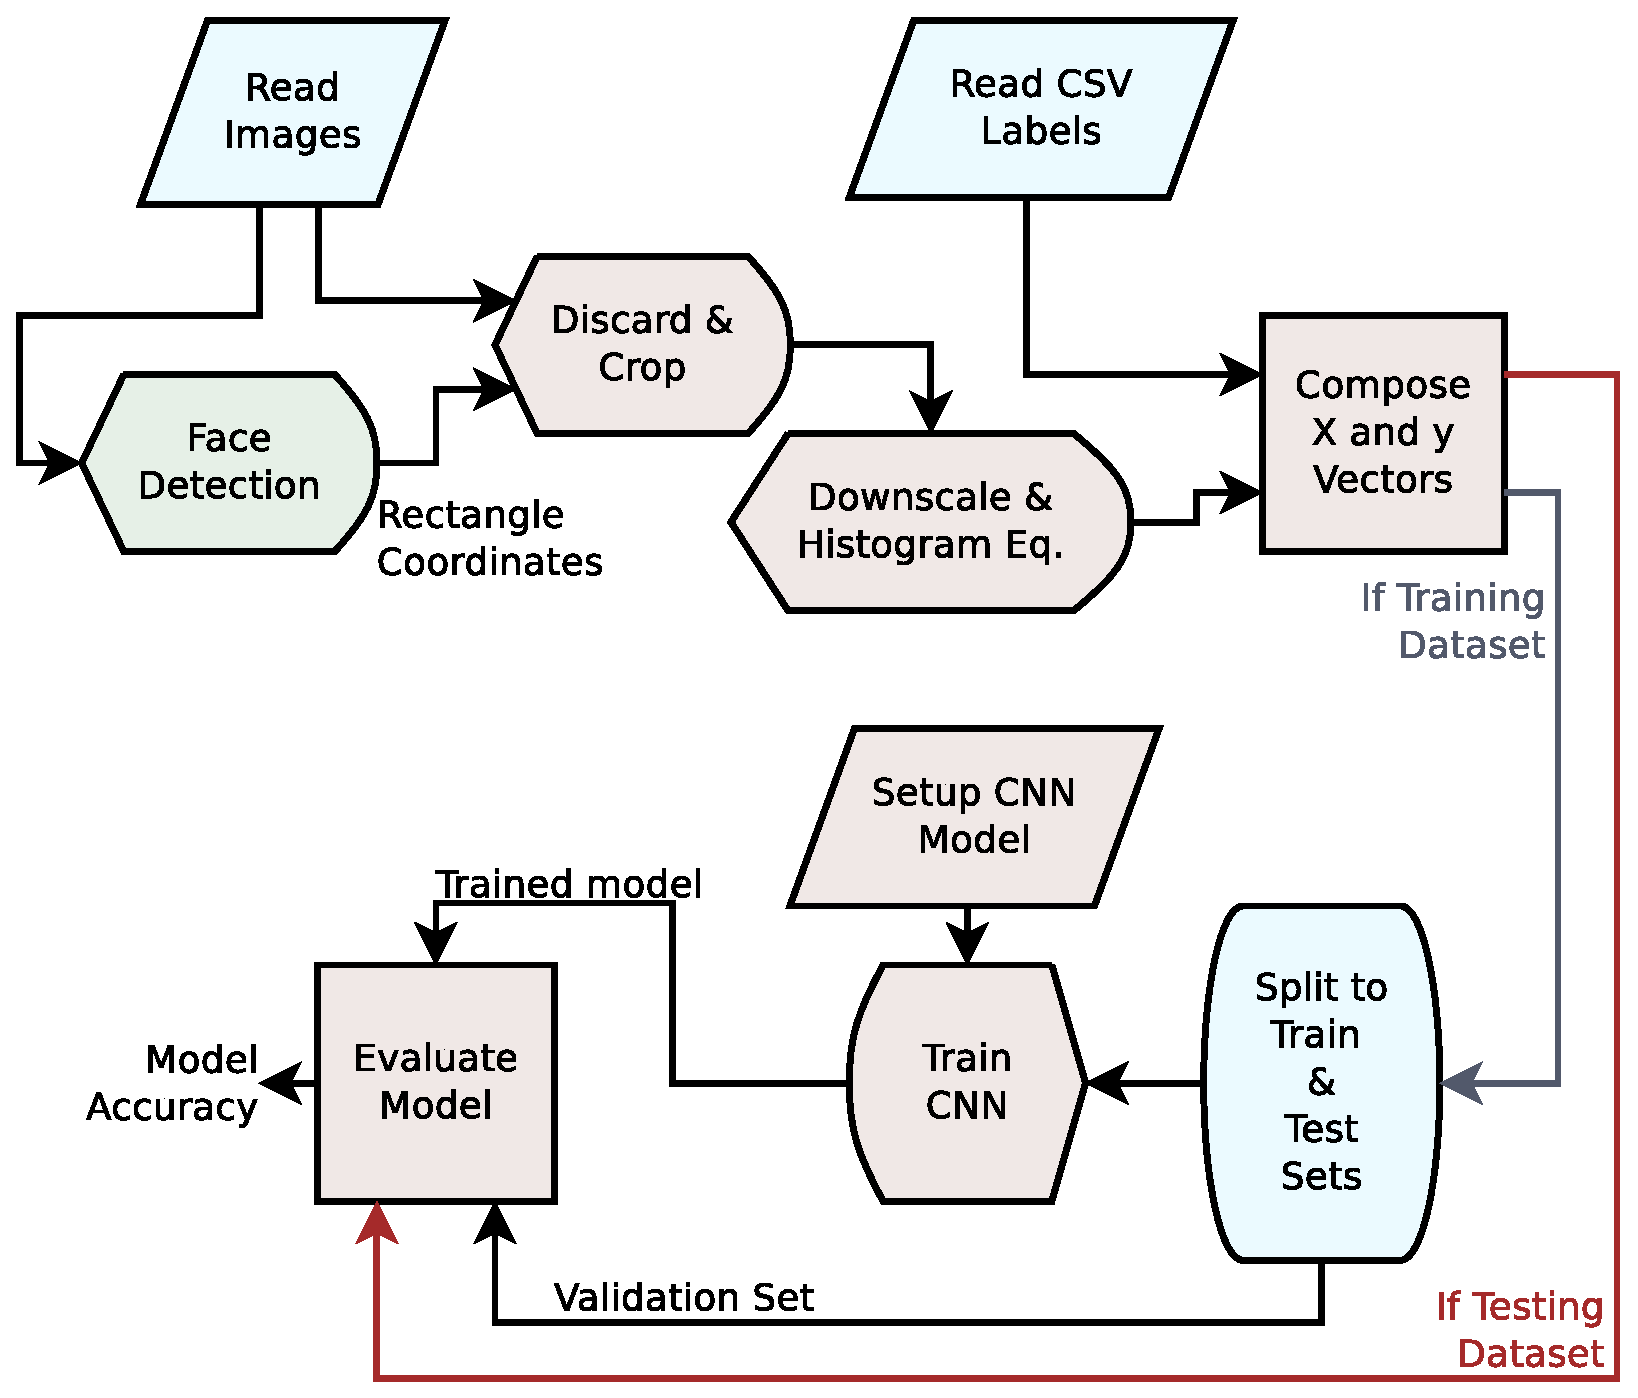
\includegraphics[width=0.48\textwidth]{graphics/A1_diagram.eps}
	\caption{Block diagram of task A1 data pipeline showing how it's proceed to train model and find model's accuracy. Blue boxes are implemented in parent class, green boxes are code that is shared with at least one other task.}
	\label{fig:block_a1}
\end{figure}

Though experimentation it was discovered that CNN performs better than other methods such as SVM and Random Forest, however the best model was SVM with poly kernel and degree of 12. This model achieved validation accuracy of 88.408\%$\pm$ 3.956\% has only around 2-3\% lower than CNN.
\autoref{fig:block_a1} describes overall data pipeline that processes dataset, trains and evaluates CNN. Face detection implementation is described in \autoref{sub:face_detect}. After acquiring face location as a rectangle position, image is read again as a grey matrix using OpenCV and cropped with defined rectangle. Further, image is downscaled to $32 \times 32$. This size has been find to be optimal size low enough to not affect model accuracy but still have fairly low dimensionality. This image is then put though histogram equalization to normalise brightness using OpenCV's \texttt{equalizeHist} method. 


CNN has been implemented using \texttt{tensorflow} and \texttt{keras} packages. \autoref{tab:a1_cnn} shows layer structure with \texttt{keras} layer names and layer arguments as parameters. 

\begin{table}[h!]
	\begin{center}
		\begin{tabular}{r|c|c} 
			\textbf{Layer name} & \textbf{Layer parameters} & \textbf{Layer activation} \\
			\hline
			Conv2D & \begin{tabular}{l@{}l@{}}Filters=8 \\ Kernel=$3\times 3$\end{tabular} & ReLU \\
			MaxPooling2D & & \\
			Conv2D & \begin{tabular}{l@{}l@{}}Filters=16 \\ Kernel=$3\times 3$\end{tabular}  & ReLU \\
			MaxPooling2D & & \\
			Flatten & & \\
			Dropout & Rate=0.2 & \\
			Dense & Units=128 & ReLU \\
			Dense & Units=2 & Softmax \\ \hline
		\end{tabular}
		\caption{CNN layer structure for task A1}
		\label{tab:a1_cnn}
	\end{center}
\end{table}

Model is compiled using \textit{adam} optimiser with \\ \texttt{CategoricalCrossentropy} loss function and accuracy metric.
Test data from train/test split is used as validation data. In addition, labels (y vector) is converted to one-hot vector using \texttt{binary\_to\_one\_hot} method defined in \textit{utils.py}. Model training has additional callback to stop training if training loss has no improvements over 3 epochs. This is done using \texttt{keras} built-in \texttt{EarlyStopping} class.

The optimal epoch size was selected 20 because as seen from \autoref{fig:a1_train_history} it is the at around the area of constant validation accuracy, meaning further training the model will not result higher accuracy; and around minima of validation loss as further training risk model to be overfitted. Training accuracy is obtained using model \texttt{evaluate} function.

\begin{figure}[htb]
	\centering
	\includegraphics[width=0.48\textwidth]{graphics/A1_train.eps}
	\caption{Task A1 CNN training history of loss and accuracy.}
	\label{fig:a1_train_history}
\end{figure}

Overall model is quite small and efficient only having 132,706 trainable parameters. Dense layer could be further reduced to decrease model complexity with some decrease in accuracy.

\subsection{Task A2: Smile classification}

Similarly to task A1, this task uses face detection method described in \autoref{sub:face_detect} to locate same face position. Face positions are cached using pickle library to save on processing time. Once again faces are read as grey images using OpenCV. Histogram equalization to normalise brightness using OpenCV's \texttt{equalizeHist} method. Features are extracted using dlib \texttt{shape\_predictor} method that is loaded 68 facial landmark predictor from \\\textit{shape\_predictor\_68\_face\_landmarks.dat} file. This method also takes face location that is computed before. 
This landmark is also processed in parallel using python's \textit{multiprocessing} library creating thread Pool. Model then further takes these landmarks as $68 \times 2$ matrix (or 136 flatten vector) and splits into test and train datasets as described in \autoref{sub:parent_class}.

\begin{figure}[htb]
	\centering
	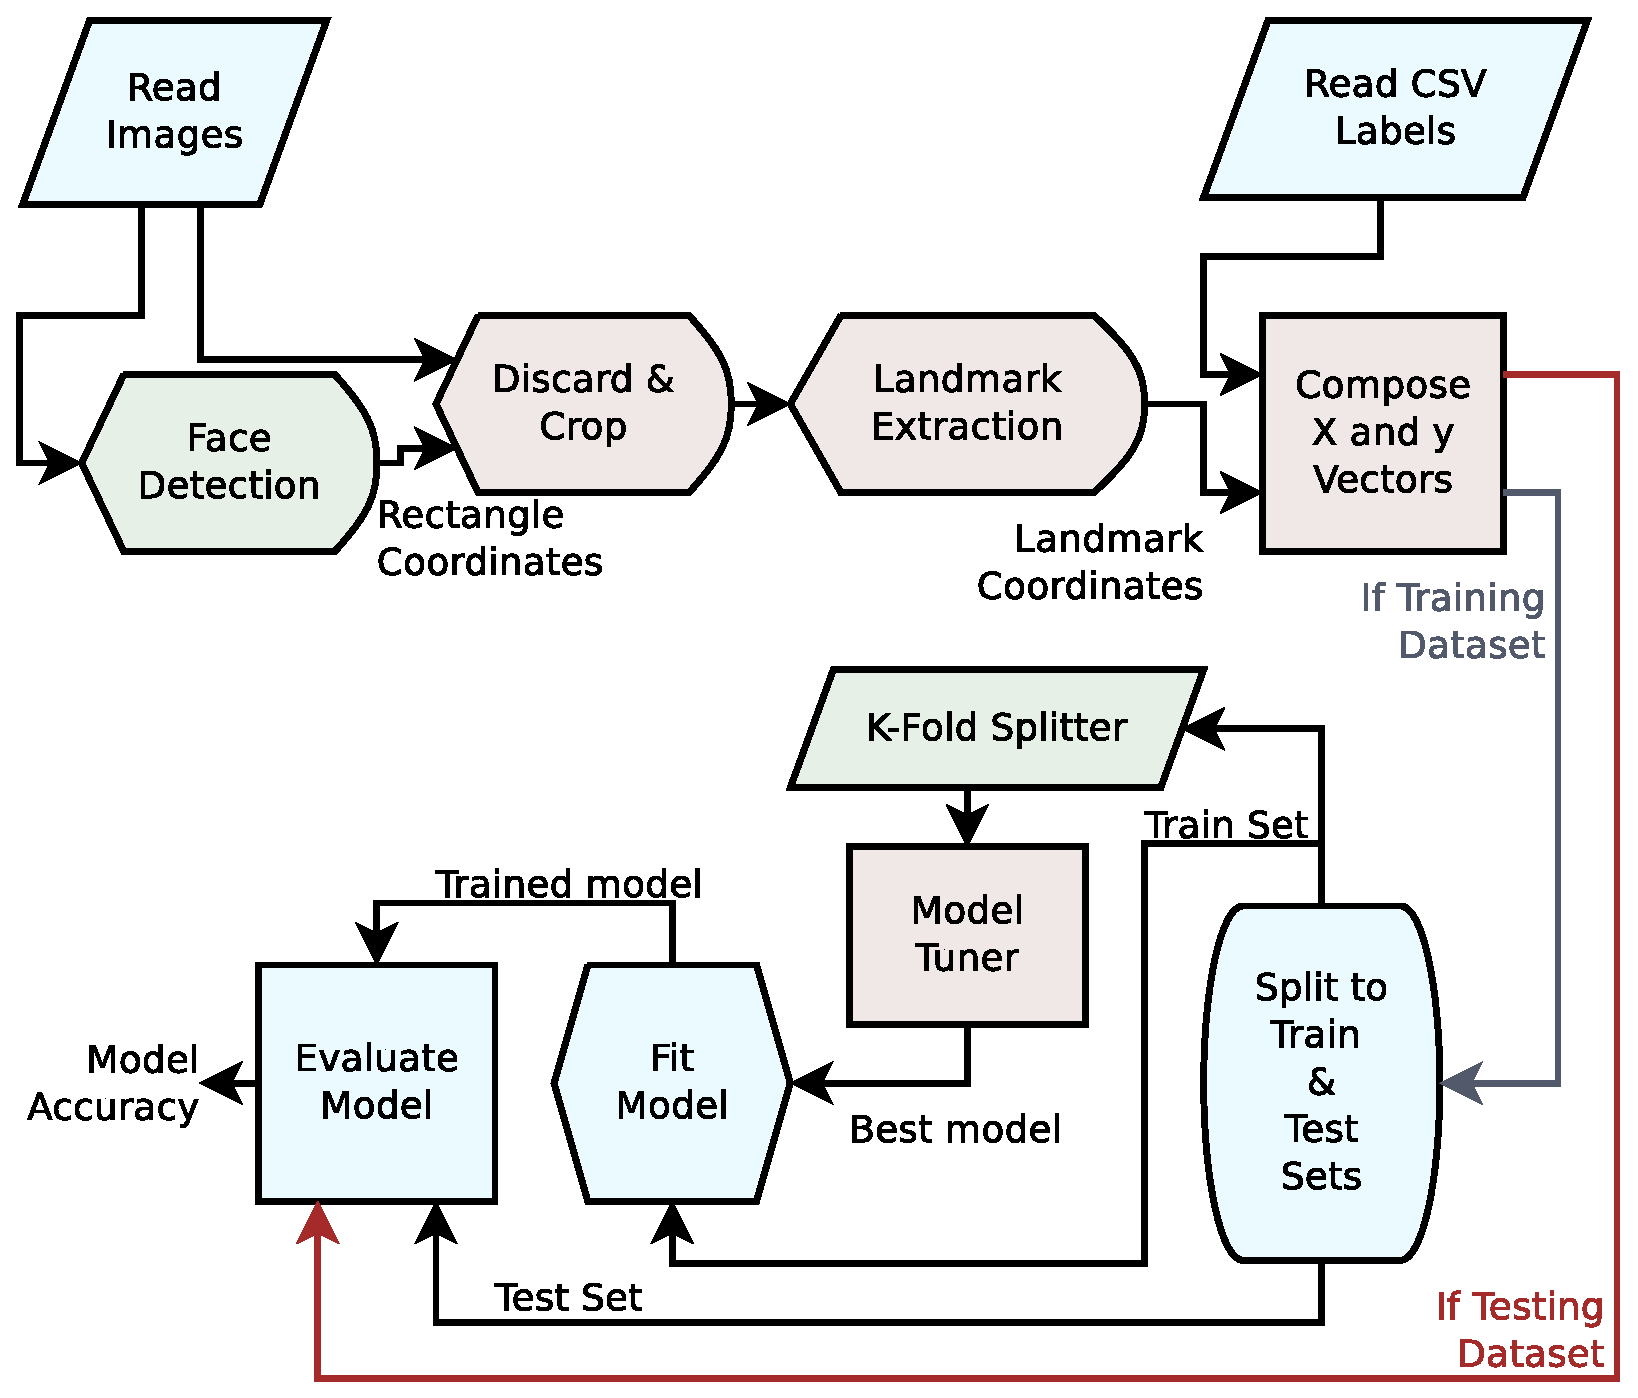
\includegraphics[width=0.48\textwidth]{graphics/A2_diagram.eps}
	\caption{Block diagram of task A2 data pipeline showing how it's proceed to train model and find model's accuracy. Blue boxes are implemented in parent class, green boxes are code that is shared with at least one other task.}
	\label{fig:block_a2}
\end{figure}

Extracted landmarks superposed on images are shown in \autoref{fig:face_features}. Here lips with landmark indices between 48 and 68 are shown in green, eyebrows with indices 17-27 in cyan, eyes with indices 36-48 in yellow, nose with indices 27-36 in blue and face shape with indices 0-17 in red points. 
\begin{figure}[htb]
	\centering
	\includegraphics[width=0.7\linewidth]{graphics/A2_landmarks.png}
	\caption{Extracted face landmarks for celebrity dataset for task A2.}
	\label{fig:face_features}	
\end{figure}

Best model is selected using method described in \autoref{sub:hypertune}. It has been discovered that best model was SVM RBF model with C parameter of 1000. Mean validation accuracy for this model was 87.468\% ($\pm$ 3.672\%). When testing whole grey downscaled to $40 \times 40$ image instead of facial landmark, lower accuracy was achieved 86.25\% with SVC model with 6th degree poly kernel and C parameter of 0.07 which has an order of magnitude higher input number. Testing lower half of the face around lips showed similar 85.27\% accuracy  with SVC 4th degree poly kernel with value C of 0.02.

To further tune hyper-parameters a grid search Cross-Validation as used with SVC model, tuning C and gamma parameters. This was implemented using \textit{sklearn} library's \texttt{StratifiedShuffleSplit} and \texttt{GridSearchCV} with 5-folds, 20\% test size and C range $10^{-2} - 10^{10}$ and gamma range $10^{-9} - 10^{3}$. Achieved accuracy was further improved to 88\%

%SVC model with 6th degree poly kernel, regularization parameter C of 0.07 yielded accuracy of 86.25\%. From \autoref{fig:face_features} it is visible that some lips are not classified correclty as model may detect chin instead. Also smile could be extracted from other features than a shape of a smile (e.g. cheeks and lip corners). As many pictures are quite noisy (e.g. there is an object in a front of mouth) these other face features might be essential to improve model accuracy. Cropping image around mouth within points 4, 9, 14, 31 and reducing gray image to 40 by 40 havepixels with SVC 4th degree poly kernel with value C of 0.02 yielded worse accuracy of 85.27\%.

\subsection{Task B1: Face shape classification}

This task as before, uses parent class described in \autoref{sub:parent_class} to load images and labels. Only preprocessing that is done is image downsampling using OpenCV \texttt{resize} function to $50 \times 50$ image, and apply histogram equalization using OpenCV's \texttt{equalizeHist} method. Data pipeline is shown in \autoref{fig:block_b1}. %Output of preprocessor is shown in \autoref{fig:b1_faces}.


\begin{figure}[htb]
	\centering
	\includegraphics[width=0.48\textwidth]{graphics/B1_diagram.eps}
	\caption{Block diagram of task B1 data flow showing how it's proceed to train model and find model's accuracy. Blue boxes are implemented in parent class, green boxes are code that is shared with at least one other task.}
	\label{fig:block_b1}
\end{figure}

Using model tuner described in \autoref{sub:hypertune} showed that best model was SVC with poly kernel, 3rd degree and normalisation parameter C=10, achieving mean cross-validation accuracy of 99.893\% ($\pm$ 0.232\%), however other models achieved similar results. 

%\begin{figure}[h]
%	\centering
%	\includegraphics[scale=0.7,interpolate]{graphics/B1_faces.png}
%	\caption{Preprocessed cartoon faces for task B1.}
%	\label{fig:b1_faces}
%\end{figure}

\subsection{Task B2: Eye colour classification}

This task is fairly similar to B1 except with an additional issue - some of the faces has non-transparent glasses meaning that it is impossible to determinate what eye colour they have. This can be viewed as natural noise in dataset. Therefore, the first step was to implement a method that remove these faces with glasses. To achieve this, dataset was examined noticing that every face and face's landmarks are almost in the same position relative to the image. This meaning that defining fixed points for instance around eye will generally outline eye in every image in the dataset. This highly biased fixed points would not be preferred in most cases, however as this method is used only to clean dataset it allows avoiding manual cleaning or developing more complicated method for this particular dataset. 

\begin{figure}[htb]
	\centering
	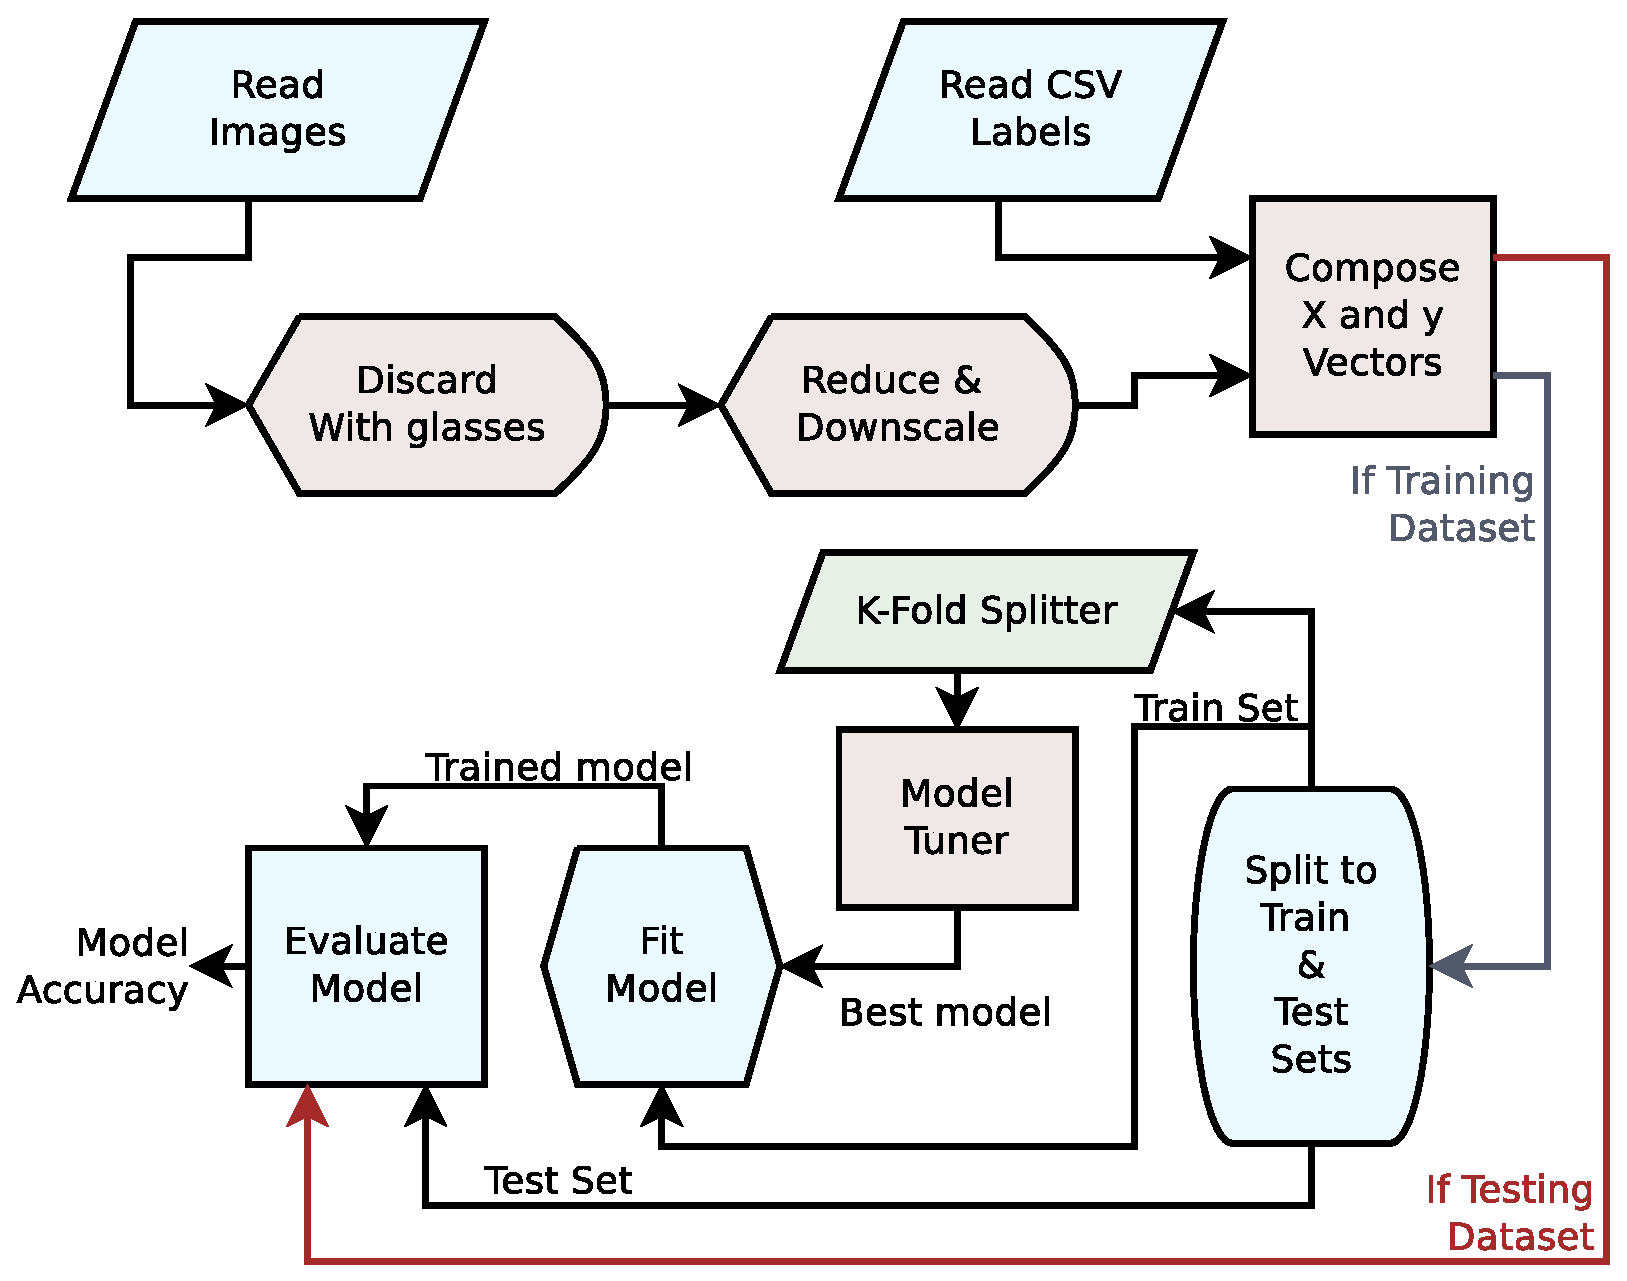
\includegraphics[width=0.48\textwidth]{graphics/B2_diagram.eps}
	\caption{Block diagram of task B2 data pipeline showing how it's proceed to train model and find model's accuracy. Blue boxes are implemented in parent class, green boxes are code that is shared with at least one other task.}
	\label{fig:block_b2}
\end{figure}

Model is implemented by using this loading images and discarding one with glasses. Implementation of this method is described in \autoref{subsub:discard_glasses}. Afterwards, image sides are cropped by 10\% as it is unlikely eyes will at the edge of the picture, and then divided vertically in half. This is done to reduce dimensionality as only one half of the face is needed to gather information about eye colour, assuming both eyes has the same colour. This cropped image is then downscaled using OpenCV function \textit{cv2.resize} with Lanczos interpolation over $8\times 8$ pixel neighbourhood to $50\times 25 \times3$ matrix. %These images can be seen in \autoref{fig:b2_output}. 
Image is stored as $X$ vector and forwarded to be split into train and test sets. 

%\begin{figure}[htb]
%	\centering
%	\includegraphics[scale=0.9,interpolate]{graphics/B2_faces.png}
%	\caption{Output images after preprocessor in task B2.}
%	\label{fig:b2_output}
%\end{figure}

To find the most optimal model and its hyper-parameters a list of models from sklearn library is tested with 10-Fold Cross-Validation using sklearn \textit{cross\_val\_score} function. Random Forest Classifier perform the best with validation accuracy of 99.41\% ($\pm$ 0.735) and estimators parameter of 300. It is implemented using sklearn \\\texttt{RandomForestClassifier} method.

\subsubsection{Discaring non-transparent glasses}
\label{subsub:discard_glasses}

In order to detect non-transparent glasses every image is cropped upper left corner of $x=240, y=180$ with size of $50\times 50$. In every image this area contain left eye with a small area around it, this can be seen in \autoref{fig:glasses_detect}. This image is further cropped at upper left corner $x=16, y=26$ with size of $20\times 20$. In \autoref{fig:glasses_detect} this patch is highlighted with green rectangle and it contains lower part of iris, slera and a bit of skin underneath eye. This smaller area is converted from RGB colour model to HSV colour space using OpenCV method \textit{cv2.cvtColor}. Mean value of HSV (hue, saturation, value) value (or brightness/darkness) component is calculated for whole area using numpy \textit{mean} method. Non-transparent glasses are detected if this mean value is below 50, which is shown as red number in every sample in \autoref{fig:glasses_detect}. As brightness component is used for this detection, eye colour will be irrelevant and also allowing to pass partly transparent and coloured glasses which are still useful for model prediction.
\begin{figure}[htb]
	\centering
	\includegraphics[width=0.48\textwidth]{graphics/B2_glasses_detect3.png}
	\caption{A number of samples showing output of detecting non-transparent glasses method.}
	\label{fig:glasses_detect}
\end{figure}



\section{Experimental Results and Analysis}
\label{sec:results}
\iffalse
This section describes and discusses your results. Addition-
ally, this section should include accuracy prediction scores on
a separate test dataset, provided by the module organizers, but
not used during your training and validation process.
We recommend you use a table to list the tasks, models
and results before analysis.
\fi

Face detection described in \autoref{sub:face_detect} managed to detect 96.62\% of faces in train dataset and 97.50\%  in test dataset. Images without detected face were excluded. 

Non-transparent glass method described in \autoref{subsub:discard_glasses} rejected 18.58\% of images from train dataset and 18.68\% from test dataset.

List of different models and hyper-parameters used to find the best model is shown in \autoref{tab:validation}.

Best model accuracy is shown in \autoref{tab:results}. Each task results have reasonable accuracy and perform with optimal performance. 

\begin{table}[h!]
	\begin{center}
		\begin{tabular}{l|c|c} 
			 & \textbf{Training Dataset} & \textbf{Test Dataset} \\
			\hline
			\textbf{Task A1} & 90.066\% & 92.000\% \\
			\textbf{Task A2} & 88.000\% & 88.800\% \\
			\textbf{Task B1} & 100\% & 99.960\% \\
			\textbf{Task B2} & 99.018\% & 99.361\% \\
		\end{tabular}
		\caption{Accuracy results for each task on training and test datasets.}
		\label{tab:results}
	\end{center}
\end{table}


\iffalse
A1:
Model SVC(C=0.1, kernel='linear') scored 0.82004 (+/- 0.02509)
Model SVC(C=1, kernel='linear') scored 0.80486 (+/- 0.04161)
Model SVC(C=10, kernel='linear') scored 0.80154 (+/- 0.03218)
Model SVC(C=0.1) scored 0.78553 (+/- 0.04053)
Model SVC(C=1) scored 0.87056 (+/- 0.03118)
Model SVC(C=10) scored 0.88132 (+/- 0.02419)
Model SVC(C=0.1, kernel='poly') scored 0.63538 (+/- 0.03010)
Model SVC(C=1, kernel='poly') scored 0.84820 (+/- 0.02973)
Model SVC(C=10, kernel='poly') scored 0.86614 (+/- 0.04160)
Model SVC(degree=6, kernel='poly') scored 0.56528 (+/- 0.02749)
Model SVC(degree=9, kernel='poly') scored 0.52829 (+/- 0.02113)
Model RandomForestClassifier(n_jobs=-1) scored 0.72896 (+/- 0.05724)
Model RandomForestClassifier(n_estimators=200, n_jobs=-1) scored 0.75793 (+/- 0.03330)
Model RandomForestClassifier(n_estimators=300, n_jobs=-1) scored 0.75269 (+/- 0.04263)
Model RandomForestClassifier(n_estimators=400, n_jobs=-1) scored 0.75269 (+/- 0.04057)
Model RandomForestClassifier(n_estimators=500, n_jobs=-1) scored 0.75462 (+/- 0.04406)
A1:
Model SVC(C=0.1, kernel='linear') scored 0.83660 (+/- 0.02675)
Model SVC(C=1, kernel='linear') scored 0.79741 (+/- 0.03202)
Model SVC(C=10, kernel='linear') scored 0.77119 (+/- 0.03087)
Model SVC(C=0.1) scored 0.78636 (+/- 0.04427)
Model SVC(C=1) scored 0.86365 (+/- 0.03844)
Model SVC(C=10) scored 0.88132 (+/- 0.03382)
Model SVC(C=50) scored 0.88187 (+/- 0.03451)
Model SVC(C=100) scored 0.88187 (+/- 0.03451)
Model SVC(C=500) scored 0.88187 (+/- 0.03451)
Model SVC(C=0.1, kernel='poly') scored 0.85979 (+/- 0.03791)
Model SVC(C=1, kernel='poly') scored 0.86476 (+/- 0.02769)
Model SVC(C=10, kernel='poly') scored 0.86476 (+/- 0.02769)
Model SVC(degree=6, kernel='poly') scored 0.87801 (+/- 0.03614)
Model SVC(degree=9, kernel='poly') scored 0.88243 (+/- 0.03772)
Model SVC(degree=12, kernel='poly') scored 0.88408 (+/- 0.03956)
Model RandomForestClassifier(n_jobs=-1) scored 0.83577 (+/- 0.03688)
Model RandomForestClassifier(n_estimators=200, n_jobs=-1) scored 0.83219 (+/- 0.03156)
Model RandomForestClassifier(n_estimators=300, n_jobs=-1) scored 0.83936 (+/- 0.03951)
Model RandomForestClassifier(n_estimators=400, n_jobs=-1) scored 0.83991 (+/- 0.03479)
Model RandomForestClassifier(n_estimators=500, n_jobs=-1) scored 0.84295 (+/- 0.03793)





Model SVC(C=0.1, kernel='linear') scored 0.99867 (+/- 0.00292)
Model SVC(C=1, kernel='linear') scored 0.99867 (+/- 0.00292)
Model SVC(C=10, kernel='linear') scored 0.99867 (+/- 0.00292)
Model SVC(C=0.1) scored 0.55440 (+/- 0.03589)
Model SVC(C=1) scored 0.90947 (+/- 0.02171)
Model SVC(C=10) scored 0.99133 (+/- 0.00708)
Model SVC(C=0.1, kernel='poly') scored 0.98813 (+/- 0.00839)
Model SVC(C=1, kernel='poly') scored 0.99773 (+/- 0.00317)
Model SVC(C=10, kernel='poly') scored 0.99893 (+/- 0.00232)
Model SVC(degree=6, kernel='poly') scored 0.99867 (+/- 0.00207)
Model SVC(degree=9, kernel='poly') scored 0.99747 (+/- 0.00437)
Model RandomForestClassifier(n_jobs=-1) scored 0.99840 (+/- 0.00373)
Model RandomForestClassifier(n_estimators=200, n_jobs=-1) scored 0.99880 (+/- 0.00303)
Model RandomForestClassifier(n_estimators=300, n_jobs=-1) scored 0.99880 (+/- 0.00278)

[2020-12-14 09:57:33,128][B1.train][INFO] Starting task B1 training ..
[2020-12-14 09:57:57,819][B2.__init__][INFO] Creating task preprocessing ..
Model SVC(C=0.1, kernel='linear') scored 0.99067 (+/- 0.01025)
Model SVC(C=1, kernel='linear') scored 0.99067 (+/- 0.01025)
Model SVC(C=10, kernel='linear') scored 0.99067 (+/- 0.01025)
Model SVC(C=0.1) scored 0.27069 (+/- 0.05624)
Model SVC(C=1) scored 0.89094 (+/- 0.03127)
Model SVC(C=10) scored 0.96193 (+/- 0.02160)
Model SVC(C=0.1, kernel='poly') scored 0.98158 (+/- 0.01225)
Model SVC(C=1, kernel='poly') scored 0.98526 (+/- 0.01076)
Model SVC(C=10, kernel='poly') scored 0.98526 (+/- 0.01076)
Model SVC(degree=6, kernel='poly') scored 0.96856 (+/- 0.01530)
Model SVC(degree=9, kernel='poly') scored 0.94793 (+/- 0.01969)
Model RandomForestClassifier(n_jobs=-1) scored 0.98797 (+/- 0.01149)
Model RandomForestClassifier(n_estimators=200, n_jobs=-1) scored 0.98895 (+/- 0.00912)
Model RandomForestClassifier(n_estimators=300, n_jobs=-1) scored 0.98969 (+/- 0.00975)
Model RandomForestClassifier(n_estimators=400, n_jobs=-1) scored 0.98895 (+/- 0.00884)
Model RandomForestClassifier(n_estimators=500, n_jobs=-1) scored 0.99091 (+/- 0.01007)
[2020-12-14 10:36:18,594][B2.test][INFO] Task B2 model achieved 99.5\% accuracy


Model SVC(C=0.1, kernel='linear') scored 0.99148 (+/- 0.00600)
Model SVC(C=1, kernel='linear') scored 0.99148 (+/- 0.00600)
Model SVC(C=10, kernel='linear') scored 0.99148 (+/- 0.00600)
Model SVC(C=0.1) scored 0.44563 (+/- 0.03179)
Model SVC(C=1) scored 0.94546 (+/- 0.01084)
Model SVC(C=10) scored 0.97167 (+/- 0.01456)
Model SVC(C=0.1, kernel='poly') scored 0.98428 (+/- 0.01047)
Model SVC(C=1, kernel='poly') scored 0.98788 (+/- 0.00749)
Model SVC(C=10, kernel='poly') scored 0.98805 (+/- 0.00732)
Model SVC(degree=6, kernel='poly') scored 0.97904 (+/- 0.01386)
Model SVC(degree=9, kernel='poly') scored 0.96479 (+/- 0.01918)
Model RandomForestClassifier(n_jobs=-1) scored 0.99279 (+/- 0.00552)
Model RandomForestClassifier(n_estimators=200, n_jobs=-1) scored 0.99345 (+/- 0.00604)
Model RandomForestClassifier(n_estimators=300, n_jobs=-1) scored 0.99410 (+/- 0.00735)
Model RandomForestClassifier(n_estimators=400, n_jobs=-1) scored 0.99361 (+/- 0.00835)
Model RandomForestClassifier(n_estimators=500, n_jobs=-1) scored 0.99345 (+/- 0.00672)

B1
Model SVC(C=0.01, kernel='linear') scored 0.87718 (+/- 0.03553)

Model SVC(C=0.1, kernel='linear') scored 0.87415 (+/- 0.03465)
Model SVC(C=1, kernel='linear') scored 0.86917 (+/- 0.03682)
Model SVC(C=10, kernel='linear') scored 0.86973 (+/- 0.03471)
Model SVC(C=0.1) scored 0.82915 (+/- 0.02573)
Model SVC(C=1) scored 0.86282 (+/- 0.02817)
Model SVC(C=10) scored 0.87524 (+/- 0.04461)
Model SVC(C=0.1, kernel='poly') scored 0.87303 (+/- 0.04269)
Model SVC(C=1, kernel='poly') scored 0.87911 (+/- 0.03400)
Model SVC(C=10, kernel='poly') scored 0.87966 (+/- 0.04121)
Model SVC(degree=6, kernel='poly') scored 0.86917 (+/- 0.03773)
Model SVC(degree=9, kernel='poly') scored 0.85290 (+/- 0.04325)
Model RandomForestClassifier(n_jobs=-1) scored 0.87331 (+/- 0.03047)
Model RandomForestClassifier(n_estimators=200, n_jobs=-1) scored 0.87331 (+/- 0.03543)
Model RandomForestClassifier(n_estimators=300, n_jobs=-1) scored 0.87469 (+/- 0.03021)
Model RandomForestClassifier(n_estimators=400, n_jobs=-1) scored 0.87525 (+/- 0.02849)
Model RandomForestClassifier(n_estimators=500, n_jobs=-1) scored 0.87580 (+/- 0.02918)

\fi

\begin{table}[h!]
	\begin{center}
		\begin{tabular}{l|c|c|c|c} 
		\textbf{Model  ~\textbackslash ~ Task}	& \textbf{A1} & \textbf{A2} & \textbf{B1} & \textbf{B2}\\
			\hline
Linear C=0.1    & 83.660 & 87.415 & 99.867 & 99.148 \\
Linear C=1      & 79.741 & 86.917 & 99.867 & 99.148 \\
Linear C=10     & 77.119 & 86.973 & 99.867 & 99.148 \\
RBF C=0.1       & 78.636 & 82.915 & 55.440 & 44.563 \\
RBF C=1         & 86.365 & 86.282 & 90.947 & 94.546 \\
RBF C=10        & 88.132 & \textbf{87.524} & 99.133 & 97.167 \\
Poly C=0.1 D=3  & 85.979 & 86.303 & 98.813 & 98.428 \\
Poly C=1 D=3    & 86.476 & 86.911 & 99.773 & 98.788 \\
Poly C=10 D=3   & 86.476 & 86.966 & \textbf{99.893} & 98.805 \\
Poly C=1 D=6    & 87.801 & 86.917 & 99.867 & 97.904 \\
Poly C=1 D=9    & \textbf{88.408} & 85.290 & 99.747 & 96.479 \\
R-Forest N=100  & 83.577 & 87.231 & 99.840 & 99.279 \\
R-Forest N=200  & 83.219 & 87.231 & 99.880 & 99.345 \\		
R-Forest N=300  & 83.936 & 87.369 & 99.880 & \textbf{99.410} \\		
R-Forest N=400  & 83.991 & 87.425 & - & 99.361 \\
R-Forest N=500  & 84.295 & 87.480 & - & 99.345 \\
		\end{tabular}
		\caption{Validation accuracy of different models and hyper-parameters. Linear, RBF and Poly note SVM kernels, Poly D value define degree parameter, R-Forest stands for Random-Forest Classifier.}
		\label{tab:validation}
	\end{center}
\end{table}

Overall, image preprocessing and models are optimised to use multiple threads to decrease computation time. In addition, models have been reduced in complexity to reduce needed computation time to train and test models with minimal penalty to accuracy. 

\section{Conclusion}
\label{sec:conc}
\iffalse
This last section summarizes the findings and suggests direc-
ions for future improvement.
\fi
In this assignment, a number of machine learning models have been tested to tackle four different tasks. Task A1 solving gender classification with celebrity face dataset was solved using custom CNN model that is tuned for optimal complexity and accuracy. CNN has achieved 3.562\% higher accuracy than SVM solution. Both tasks A1 and A2 use Haar Classifier and Dlib library's face detector to detect and extract faces from images. Task A2 further uses 68 facial landmark detector to extract landmark coordinates and use them with SVM model to classify if person is smiling or not. 

With task B1 SVM performed exceptionally well with minimal image preprocessing of histogram equalization and downsampling. 

Task B2 needs to classify cartoon character's eye colours which required additional preprocessing due to dataset containing noise. This noise is seen as non-transparent glasses that obstruct eyes. A manual detector was successfully written to remove images with these classes and model was further processed with Random Forest Classifier model achieving high accuracy and efficiency. 

For future work, both tasks A1 and A2 could implement additional facial rotation and alignment and provide a number of differnet regions of faces for task A1 CNN model to see any performance increase, as discussed in literature review. As well, to further increase computation performance for CNN, model with lower accuracy data representation (e.g. 16bit float) could be used to see performance improvements. Task B1 might also benefit from reducing image resolution or apply Principal Component Analysis (PCA).

\vfill\pagebreak

\bibliographystyle{IEEEbib}
\bibliography{refs}

\end{document}